%%%%%%%%%%%%%%%%%%%%%%%%%%%%%%%%%%%%%%%%%%%%%%%%%%%%%%%%%%%%%%%%%%%%%%%%%%%%%%%%
% setup.tex
% Main tex file for setup and content collocation
% For the use of University of Amsterdam
% Information Systems and Data Science students
% Adapted by Riccardo Fiorista (riccardo.fiorista@proton.me)
%%%%%%%%%%%%%%%%%%%%%%%%%%%%%%%%%%%%%%%%%%%%%%%%%%%%%%%%%%%%%%%%%%%%%%%%%%%%%%%%

% Options:
% Choose one of:
%% `is` - Information Systems
%% `ds` - Data Science 
% Add (separated by `,`):
%% `nolinenumbering` - If you want to remove line numbering on submission
%% `draftmargins` - If you would like to give your reviewer more space for comments
%% `nofrontpicture` - If you do not wish to have a graphic on your front-page
%% `nofirstcompanypicture` - If you do not wish to have a graphic on your front-page
%% `nosecondcompanypicture` - If you do not wish to have a graphic on your front-page
\documentclass[ds]{mscthesis}

%%%%%%%%%%%%%%%%%%%%%%%%%%%%%%%%%%%%%%%%%%%%%%%%%%%%%%%%%%%%%%%%%%%%%%%%%%%%%%%%
% DOCUMENT METADATA
%%%%%%%%%%%%%%%%%%%%%%%%%%%%%%%%%%%%%%%%%%%%%%%%%%%%%%%%%%%%%%%%%%%%%%%%%%%%%%%%

% Thesis related entries
\title{The Impact of Anonymization Techniques on Machine Learning Accuracy for Energy cost}
%\subtitle{Fill In Your Sub-Title}

% Date on which your thesis is submitted
\date{University of Amsterdam, UvA DD.MM.YYYY}

% 4-5 keywords should do the trick. They should ideally be phrases of 2-4 words or single words.
\keywords{keywords, belong, here, with, commas, like, this}

% Author data
\authorname{Abraham Foto}
\authorid{12489727}
\authoremail{abraham.foto@student.uva.nl}

% Supervisors
\uvasupervisorname{Dr.Ana Oprescu}
\uvasupervisoraffiliation{Assistant professor}
\uvasupervisoremail{a.m.oprescu@uva.nl}

% Comment if you do not have an external supervisor
% \externalsupervisorname{External Supervisor} \externalsupervisoraffiliation{External Supervisor}
% \externalsupervisoremail{supervisor@company.nl}

% % Uncomment and fill paths if you want to add custom images
% %% Figure size suggestions (in general it's best to render them from SVGs):
% %% 3000x3000 @ 240dpi for all three
% \titlepicturepath{}
% \firstcompanypicturepath{}
% \secondcompanypicture{path}

%%%%%%%%%%%%%%%%%%%%%%%%%%%%%%%%%%%%%%%%%%%%%%%%%%%%%%%%%%%%%%%%%%%%%%%%%%%%%%%%
% CONTENT
%%%%%%%%%%%%%%%%%%%%%%%%%%%%%%%%%%%%%%%%%%%%%%%%%%%%%%%%%%%%%%%%%%%%%%%%%%%%%%%%

\begin{document}

\pagestyle{plain}
\setcounter{page}{0}

\maketitlepage
\fixemptypage

\begin{abstract}
% A summary of results should be included. Avoid citations. Maximum length is 200 words.
%Our results show that the choice of anonymization technique can have a significant impact on the accuracy of the machine learning models. In particular, k-anonymity and l-diversity can result in a significant loss of accuracy, while t-closeness has a more limited impact on accuracy. These findings have important implications for the use of anonymization techniques in the context of machine learning research.
\end{abstract}

\maketitle

%\section*{Github Repository}
%\url{https://github.com/you/your_awesome_thesis_repo}

% Sections; Try to stick to this setup but you can comment each section\\
\section{Introduction}
\label{sec:introduction}
Artificial intelligence (AI) and Machine Learning (ML) architectures have been applied to several applications that involve sensitive data, where a  guarantee  of  users’  data  privacy  is  required \cite{arous2023exploring}. They are increasingly and intensively being utilized in fields such as healthcare, finance, retail, manufacturing, transportation, agriculture and many more sectors and are found to be more efficient and effective in foresting, optimization, in tackling complicated issues, in making data driven decisions and providing with more insight to business\cite{bigbookml}. This can lead to improved productivity, financial savings, and novel insights across numerous industries. To achieve maximum accuracy using machine learning, ML models need to be trained in amount and quality of training data. However, training ML models in a large and quality data could result in exposing sensitive private data\cite{soykan2022survey} as a result could lead to the undesirable issue of privacy concerns.\\
Despite the fact that the existence of data privacy laws such as the GDPR in the EU and the CCPA in California aimed at preventing privacy violations and set standards for the gathering, use, and processing of personal data of EU and Canada citizens \cite{goldsteen2022anonymizing}, consumers' privacy is still often compromised by hackers, businesses, and governments\cite{newman2020gdpr}. In general, processing personal information is banned unless it is specifically permitted by law, or the data subject has given consent or is anonymized or synthetic data\cite{Einwilligung}. According to \cite{xiangmin2010research}, it is claimed that we can identify about 60 percent of individuals using only their date of birth, zip code, and gender. To overcome the issue of privacy and gain maximum accuracy, there is a desire to use ML/AI approaches data to transform sensitive data into valuable information while adhering to the consent of the parties involved or use synthetic data. Both GDPR and CCPA doesn't apply to anonymized or synthetic data\cite{soykan2022survey, oprescu2022energy}. Therefore, anonymized or synthetic data can be shared with a third party or can be mode publicly available for different educationally and research analysis purpose with out consent.\\
Data anonymization is the process of protecting sensitive or private information by removing or encoding identifiers that connect specific people to the data \cite{}.\todo{REF} In the processes of data anonymization, one need to make sure that the statistical conclusions drawn from anonymized data should have the same meaning to the one drawn fro  the original data. \\
the statistical conclusions drawn from it shouldn't be influenced by an individual's contribution.
Anonymization techniques are  common practice in data mining and machine learning research to protect the privacy of individuals whose data is being analyzed. However, these techniques can have a negative impact on utility of the data\cite{rodriguez2020contribution} and accuracy of machine learning, which rely on the availability of accurate and complete data to make predictions\cite{}.\todo{REF}

k-anonymity and Differential Privacy are widely used anonymization technique is proposed by \cite{sweeney2002k} and \cite{dwork2006differential} respectively. Both techniques are believe to be the most effective privacy guarantee now available, provides strong, demonstrable guarantees for preserving privacy\cite{liu2019k}. While k-anonymity approaches assume a trusted aggregator of the data, Differential Privacy adds noise in the data to mask the real value \todo{ref}.\\

As of now, both k-anonymity and Differential Privacy are  implemented in different architecture of ML as PETs. \cite{wimmer2014comparison} suggested that certain machine learning algorithms are more suited to use with k-anonymity techniques than others and \cite{rodriguez2020contribution} added that it is unclear how privacy protection techniques actually affect the usefulness of data.To the best of our concern there is a limitation or not an empirical evaluation on the impact of PETs in ML models accuracy. 
%Privacy Enhancing Techniques(PETs) has been the subject of many research topics for many years, techniques like k-anonymity and Differential privacy are proposed as a powerful methods for data privacy\cite{rodriguez2020contribution,oprescu2022energy,wimmer2014comparison,chang2023privacy}. 
%Anonymization is degffination.......

%The common way to protect privacy is to use K-anonymity in data publishing. https://ieeexplore.ieee.org/abstract/document/5462427

In this paper, we investigate the impact of anonymization techniques on the accuracy of machine learning models using the  two commonly used anonymization techniques: k-anonymity and  Differentially Private. We evaluate the performance of these techniques on two different machine learning models: k-nearest neighbours, Logistic Regression and Neural networks. Therefore, the main research question would be:
\begin{center}
    \textbf{ \textbf{(RQ)The impact of anonymization techniques on machine learning model's accuracy and energy consumption?}}
\end{center}

Further, this paper will tries to broaden the research by \cite{oprescu2022energy, hoyos2020contribution} by including more PETs and more ML models and energy consumption. Both suggested that it is worth of studying the impact of PETs on ML accuracy.

This paper is structured as follows: Section II reviews on several  anonymization  techniques.  Section  III  explains  the  existing   privacy-preserving   techniques.   Next,   Section   IVdiscusses  privacy  preservation  in  database  fields.  Lastly,  Section  V  presents  the  conclusion  and  future  works.  The  intention  of  this  review  is  to  compare  five  anonymization  techniques in a situation where the data is about to be shared with other organizations or entities.\todo{ref}

%Mention scientific context/field, problem statement, research gap and (sub) research question(s). 
%Write your introduction here. It should be immediately clear how your proposed contribution is scientifically relevant and fills the research gap.
% \TODO{This is a TODO} This is a test citation \cite{Gruber1995}

%Towards the end of the introduction, you should also add your \textit{preliminary} \textbf{reasearch questions (RQ)} here. You may want to state your main RQ like this:

%\noindent\textit{To what extent can a master thesis template enhance the quality of the final thesis?}\REMARK{This is a remark}

%You can then list the sub-questions as:
%\begin{itemize}
%    \item How does the structure of the template influence the final grading?
%    \item To what extent is textual guidance sufficient for structured working?
%    \item \dots
%\end{itemize}

%As the amount of data being generated and collected continues to grow, there is an increasing need to protect the privacy of individuals whose data is being analyzed. Anonymization techniques are often used to achieve this goal, by removing or obfuscating identifying information from data sets. However, these techniques can also have a negative impact on the accuracy of machine learning models, which rely on the availability of accurate and complete data to make predictions. The goal of this paper is to investigate the impact of anonymization techniques on the accuracy of machine learning models.
%Machine Learning (ML) architectures have been applied to several applications that involve sensitive data, where as  guarantee  of  users’  data  privacy  is  require \cite{arous2023exploring}. 
\section{Related Work}
\label{sec:related_work}
% Your work needs to be grounded and compared to earlier work and the state-of-the-art. Start the section with announcing the research gap and also end with the research gap. Consider using hypotheses. 
\cite{goldsteen2022anonymizing,wimmer2014comparison} claimed that ML model trained on an anonymized data results in degraded accuracy. Further \cite{wimmer2014comparison} pointed out that certain  machine  learning  algorithms accuraccy is impacted by PETs, K-Anonymity, \todo{Check the importance of the claims with TA}; in accordance with his claim
 \cite{arous2023exploring} tried to address accuracy loss leading to sub-optimal  privacy/utility  trade-offs, focusing on the hyperparameter space of the model impact on the loss of accuracy.\\ To the best of research and knowledge, there is/are no empirical comparative research on PETs, this section will provide a overview of the techniques and concepts implemented.
% The related work section is not a a background section. If you want to explain techniques, it is possible to have a background section after the Related Work section. Background should only be added when it has benefit for an informed audience. It is not common to use a background section. 
\subsection{Privacy issues in the era of big data}
The era of big data has brought significant benefits in terms of the ability to extract insights from large datasets\cite{zhang2019brief}. However, it has also raised concerns about privacy issues\cite{liu2019k}. With the increasing amount of data being collected, processed, and analyzed, there is a risk that sensitive information could be exposed or misused. This can lead to the exposure of personal information, such as financial data, health records, or social security numbers\cite{murthy2019comparative}.\\
To address these privacy issues, there needs to be a focus on building fair and unbiased algorithms that do not reveal personal information or other sensitive information while maintaining the usability of the original data\cite{murthy2019comparative,sweeney2002k} .
\subsubsection{ k-anonymity}
K-anonymity is a privacy protection technique used in data mining and statistical analysis. It ensures that individuals cannot be identified by their personal information in a dataset by grouping them with others who share similar characteristics.\todo{Ref} This helps to prevent the disclosure of sensitive information and protect the privacy of individuals. Is there anything else I can assist you with?\\
In recent years, a new definition of privacy called k-anonymity has gained popularity \cite{sweeney2002k,murthy2019comparative}. It has been implemented on protect privacy in medical data \cite{el2008protecting}.
K-anonymity was first proposed on [4] and states that in order to achieve k-anonymity, the information for each person contained in the released dataset cannot be distinguished from at least �� − 1 individuals whose information also appear in the released dataset.

There are two methods for or achieving k-anonymity: suppression and generalization. The former approach replaces some of the entries with an asterisk ’*’, while the latter one groups the entries into categories.
\todo{how k works}
\subsubsection{Differential privacy}
Differential privacy (DP) is an advanced data anonymization method or technique that introduces basic mathematical definitions to enable privacy measurement (DPSGD)\cite{arous2023exploring,ponomareva2023dp,horlboge2022still} , but DPSGD suffers from a significant accuracy loss that results in insufficient privacy/utility trade-offs \todo{ref}. \cite{arous2023exploring} and further claimed that with improving hyperparameters of the learning algorithm, they were able to achieve a higher accuracy without changing learning procedure. \cite{singh2022privacy} proposed a novel approach of differential privacy to in cloud architecture and results show that PPMD ensures high accuracy, precision, recall, and F1-score improvement up to 29 percent over the existing works.\\
To protect the privacy of individuals, differential privacy adds noise in the data to mask the real value, and thus, making it private. By doing this, we hide the individual’s identity with little to no impact on the utility of the data. This means that the statistical outcomes from the dataset should not be influenced by an individual’s contribution since the data represents the characteristics of an entire population. Let D and D’ represent two distinct neighbouring datasets differing in only one data set. Differential privacy states that to secure the private attributes in a given dataset by adding a noise ��, we cannot predict whether a particular entry exists in the database or not\todo{Ref}. \todo{How DF works}
 
\subsection{Machine Learning}
\begin{itemize}
    \item Neural Networks:
    Neural Networks are one of the most advanced and complex algorithms in machine learning, which can only handle numeric data. NN is a computational technique which is modeled after the human brain’s neural pathways \cite{wimmer2014comparison} and is known for requiring high processing time.
    \item Logistic Regression:
    
    \item k-Nearest Neighbour (KNN)
    
\end{itemize}

\section{Methodology}
\label{sec:methodology}
% Focus on what you add to the existing method. Explain what you will do and why (and how). Do not forget to characterize your research design. There should be a sub-section on the evaluation. 
%For DS students, this normally means using manually labelled or ground truth data. For IS students, it is not always needed to have a separate methodology section. You can also integrate the approach with the results in one section. It depends on your type of research what is best fitting.
\subsection{Data}
\label{data}
To investigate the impact of anonymization techniques on the accuracy of machine learning models, we used two real data sets: Early stage diabetes risk prediction\cite{ucidiabetes} and adult\cite{UCIAdultDataset}, which are both publicly available on the UCI Machine Learning Repository. The data set in question has been widely used to evaluate binary classifiers and privacy preserving techniques as they contains demographic information about individuals\cite{rodriguez2020contribution,oprescu2022energy}. These dataset is a common benchmark for evaluating machine learning models in the area of privacy-preserving data analysis\todo{ref}. For the details about the data referee to appendix \ref{Early Stage Diabetes}.\\
The use of early stage diabetes data for privacy-enhancing techniques depends on various factors, including the nature and sensitivity of the data, the privacy risks involved, and the specific technique being used.\todo{ref}In general, medical datasets, including early stage diabetes data, are considered to be highly sensitive due to the personal and sensitive nature of the information they contain. As such, they require strong privacy protections to ensure that individuals' privacy is not compromised. Privacy-enhancing techniques, such as differential privacy, k-anonymity, and secure multi-party computation, can be used to protect the privacy of individuals in medical datasets while still allowing useful analysis to be performed on the data.\todo{ref}.\\
The adult data set, which is also known as the Census Income dataset, taken in 1994 has 48,842 instances with 14 attributes and a labeled target attribute, salary. it includes attributes such as age, education level, occupation, marital status, and income. The goal of the dataset is to predict whether an individual's income is greater than or equal to 50,000 per year based on their demographic information\ todo{ref}. \\
First classify the data using ML algorithm on the original data set, un-anonymized data\ref{fig:Machine Learning Process And Scenarios} and then the same algorithms are applied to the identical(the same) data after it has been anonymized using the privacy framework \ref{fig:anonymization}. This approach is useful in cases where it is necessary to protect the privacy of individuals in the data, but also important to maintain the utility of the data for analysis or other purposes\cite{wimmer2014comparison}.\\
\subsubsection{Data Pre-Processing}
Data pre-processing is a technique used to convert raw data into a clean or ready dataset \cite{han2012}. The data pre-processing phase is crucial in the learning process of the algorithm, because different algorithms require different data pre-processing \cite{han2012}.  
\subsubsection{Initial data exploration and cleaning}
\begin{itemize}
    \item Early stage diabetes risk prediction: This dataset comprises 520 records which were collected using direct questionnaires from the patients of Sylhet Diabetes Hospital in Sylhet, Bangladesh in the year 2020. It contains binary and real features related to medical conditions and characteristics of patients admitted to the Sylhet Diabetes Hospital. It is a balanced dataset with 16 features in total including the age and gender of the participants. The data we consider as private attributes for our analysis is only the age though.\todo{ref}.
\end{itemize}
\subsubsection{Data anonymization and Data transformation}
\begin{itemize}
    \item k-anonymity: The first step in implementing was to identify the attributes as identifier, non-identifier and quasi-identifier (somewhat identifying) \todo{ref}. The attributes we use as quasi-identifiers are age, education, marital-status, sex, capital-gain, and hours-per-week of the Adult dataset while ..... are identied as a quasi-identifiers in Early stage diabetes risk prediction.
    \item Differential Privacy:
\end{itemize}
\subsection{Framework(setup) Experiment}
\begin{figure}[htb!]
    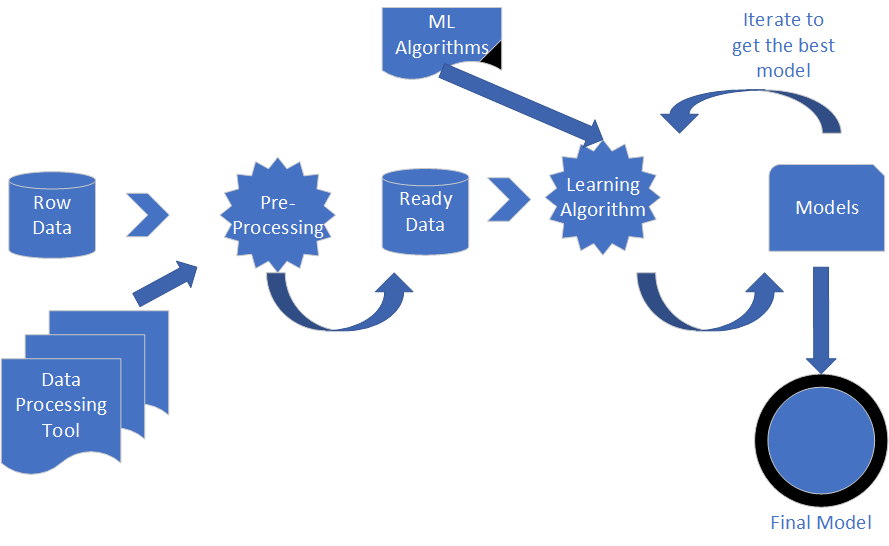
\includegraphics[scale=0.325]{media/framework/ml process.png}
    \caption{Machine Learning Process And Scenarios}
    \label{fig:Machine Learning Process And Scenarios}
    \vspace{0mm}
\end{figure} 
\begin{figure}[htb!]
    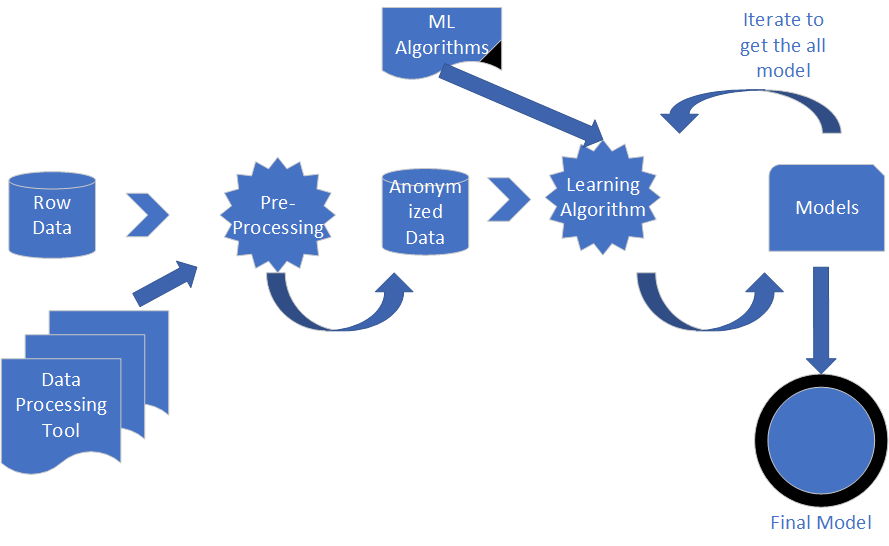
\includegraphics[scale=0.325]{media/framework/anonymization framwork.png}
    \caption{Anonymization Process}
    \label{fig:anonymization}
    \vspace{0mm}
\end{figure} 
\subsubsection{Evaluation Matrics}
\subsubsection{Results}
% It is possible to use a separate section for the Experimental Setup, which then focuses on all settings used in your experiments. It also possible to address the settings in a sub-section under Methodology. 




 
\section{Results}
\label{sec:results}
% Give the outcomes for each research question in the form of a table or graphic (with caption).
Write about your results here. Good captions to tables and/or figures are key.

% Sometimes,  especially  if  you  have  quite  different experiments or research  questions,  it makes sense to interleave the experimental setup and the results sections, so the reader does not get lost. It is then helpful to structure clearly in (sub)subsections.

Our results show that the choice of anonymization technique can have a significant impact on the accuracy of machine learning models. In particular, k-anonymity and l-diversity can result in a significant loss of accuracy, while t-closeness has a more limited impact on accuracy. This was true for both the decision tree and neural network models, and for both the medical and financial data sets.

%\section{Discussion}
\label{sec:discussion}
% Compare your results with the state-of-the-art and reflect upon the results and limitations of the study. You can already hint at future work to which you come back in the conclusion section.
Write your discussion here. Do not forget to use sub-sections. Normally, the discussion starts with comparing your results to other studies as precisely as possible. The limitations should be reflected upon in terms such as reproducibility,  scalability,  generalizability,  reliability  and  validity. It is also important to mention ethical concerns.
%\section{Conclusion}
\label{sec:conclusion}
% Answer each research question and address how the limitations of the study qualify the conclusion.
Write your conclusion here. Be sure that the relation between the research gap and your contribution is clear. Be honest about how limitations in the study qualify the answer on the research question.

The results of our study suggest that the choice of anonymization technique should be carefully considered in the context of machine learning research, as it can have a significant impact on the accuracy of the resulting models. While k-anonymity and l-diversity are widely used in

\bibliographystyle{ACM-Reference-Format}
\bibliography{bibliographies/references}

\newpage
% You can choose whether you prefer a single or double column appendix.
% Whatever you choose, you will need to stick to it throughout the appendix.
% For double column style, comment the next line.
\onecolumn

\appendix
\begin{appendices}
\section{}
\subsection{Data set}
Describes the main characteristics of the data sets tested in our experiments. The 14 attributes of the Adult data set are consists of both Categorical and Integer data types.
\begin{table}[H]
\label{Early Stage Diabetes}
    \centering
    \begin{tabular}{|c|c|c|c|c|}
    \hline
    \textbf{Data set}  &  \textbf{# of instance } &  \textbf{Associated Tasks} &  \textbf{Missing Values?} &  \textbf{# of attributes }\\
    \hline
    Adult\cite{UCIAdultDataset} &  48842  &  Classification &  14  &  yes \\
    \hline
      Early Stage Diabetes Dataset \cite{ucidiabetes}&  0.368 &  0.36 &  0.36 &  0.36 \\
    \hline
    subset data  &  0.47 &  0.36 &  0.36 &  0.36  \\
    \hline
    \end{tabular}
    \caption{ Description of the Data sets Used to Evaluate the Impact Anonymzation}
    \label{tab:Data set}
\end{table}

\subsection{First Appendix}
Shows the machine learning algorithms employed for each dataset.
\begin{table}[H]
\label{Early Stage Diabetes}
    \centering
    \begin{tabular}{|c|c|c|}
    \hline
    \textbf{ML algorithms}  &  \textbf{Type} &  \textbf{Name}\\
    \hline
    ANN &  Classification  &  -  \\
    \hline
      LR &  regression &  - \\
    \hline
    KNN  &  Clustering &  - \\
    \hline
    \end{tabular}
    \caption{Machine learning algorithms used in our experimental evaluation}
    \label{tab:ML}
\end{table}

\label{sec:apx:first_appendix}

\end{appendices}


\end{document}

%%%%%%%%%%%%%%%%%%%%%%%%%%%%%%%%%%%%%%%%%%%%%%%%%%%%%%%%%%%%%%%%%%%%%%%%%%%%%%%%
%%%%%%%%%%%%%%%%%%%%%%%%%%%%%%%%%%%%%%%%%%%%%%%%%%%%%%%%%%%%%%%%%%%%%%%%%%%%%%%%